\subsection{Results for Heading}
%\label{subsec:direction_results}
%\vspace{10pt}

Figure~\ref{fig:var_direction} represents the $p$-values for the Wilcoxon signed-rank test on actual and predicted values across $k$-fold validation datasets for the heading in the $k$-fold testing datasets using different RNN models, and forecasting times. Darker colors in grayscale represent a higher $p$-value in a range from $0$ to $1$. The values on the secondary diagonal are all equal to $1$ and black because models equal themselves.

\begin{figure}[!ht]
	\centering
	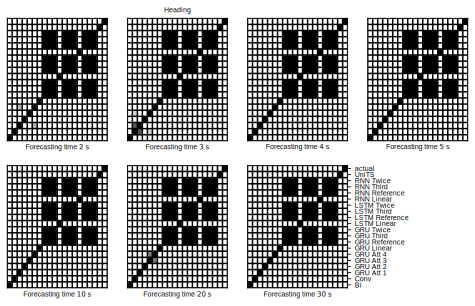
\includegraphics[width = 0.99 \linewidth]{var_direction.pdf}
	\caption{The $p$-values for the Wilcoxon signed-rank test on actual and predicted values across $k$-fold validation datasets for the heading in the $k$-fold testing datasets using different RNN models, and forecasting times. Darker colors in grayscale represent a higher $p$-value in a range from $0$ to $1$. The values on the secondary diagonal are all equal to $1$ and black because models equal themselves.}
	\label{fig:var_direction}
\end{figure}

Figure~\ref{fig:best_R2_val} contains the average $R^{2}$ (\%) across $k$-fold testing datasets using different validation datasets for all variables estimated in nested $k$-fold cross-validation by different RNN models, and forecasting times.

\begin{figure}[!ht]
	\centering
	\includegraphics[width = 0.99 \linewidth]{best_R2_val.pdf}
	\caption{The average $R^{2}$ (\%) across $k$-fold testing datasets using different validation datasets for all variables estimated in nested $k$-fold cross-validation by different RNN models, and forecasting times.}
	\label{fig:best_R2_val}
\end{figure}

The average $R^{2}$ (\%), with standard deviation in brackets, across $k$-fold validation datasets for the heading estimated on the $k$-fold testing datasets by different RNN models, and forecasting times is listed in Table~\ref{tab:best_direction_R2}.

\begin{table}[!ht]
	\centering
	\resizebox{\linewidth}{!}{
		\begin{tabular}{|c|c|c|c|c|c|c|c|}
			\hline
			Model & $2$ $s$ & $3$ $s$ & $4$ $s$ & $5$ $s$ & $10$ $s$ & $20$ $s$ & $30$ $s$ \\ \hline
			\multirow{2}{*}{Conv} & $81.67\%$ & $77.24\%$ & $\mathbf{73.59\%}$ & $\mathbf{70.18\%}$ & $57.0\%$ & $41.68\%$ & $33.83\%$ \\
			 & ($1.68\%$) & ($2.1\%$) & \textbf{(}$\mathbf{2.03\%}$\textbf{)} & \textbf{(}$\mathbf{2.35\%}$\textbf{)} & ($2.73\%$) & ($3.38\%$) & ($3.72\%$) \\ \hline
			\multirow{2}{*}{RNN Linear} & $\mathbf{86.11\%}$ & $\mathbf{79.12\%}$ & $72.83\%$ & $68.34\%$ & $51.75\%$ & $28.44\%$ & $16.2\%$ \\
			 & \textbf{(}$\mathbf{1.3\%}$\textbf{)} & \textbf{(}$\mathbf{2.11\%}$\textbf{)} & ($2.27\%$) & ($2.23\%$) & ($3.08\%$) & ($3.04\%$) & ($4.48\%$) \\ \hline
			\multirow{2}{*}{UniTS} & $77.09\%$ & $74.0\%$ & $71.12\%$ & $68.39\%$ & $\mathbf{57.72\%}$ & $\mathbf{44.0\%}$ & $\mathbf{34.98\%}$ \\
			 & ($1.99\%$) & ($2.25\%$) & ($2.42\%$) & ($2.55\%$) & \textbf{(}$\mathbf{2.76\%}$\textbf{)} & \textbf{(}$\mathbf{3.21\%}$\textbf{)} & \textbf{(}$\mathbf{3.79\%}$\textbf{)} \\ \hline
		\end{tabular}
	}
	\caption{The average $R^{2}$ (\%), with standard deviation in brackets, across $k$-fold validation datasets for the heading estimated on the $k$-fold testing datasets by different RNN models, and forecasting times.}
	\label{tab:best_direction_R2}
\end{table}

The Conv model achieved the highest $R^{2}$ (\%) for heading, and a forecasting time of $4$, and $5$ $s$ with average values and standard deviation (in brackets) that equal $73.59$\% ($2.03$\%), and $70.18$\% ($2.35$\%) respectively.

The RNN Linear model achieved the highest $R^{2}$ (\%) for heading, and a forecasting time of $2$, and $3$ $s$ with average values and standard deviation (in brackets) that equal $86.11$\% ($1.3$\%), and $79.12$\% ($2.11$\%) respectively.

The UniTS model achieved the highest $R^{2}$ (\%) for heading, and a forecasting time of $10$, $20$, and $30$ $s$ with average values and standard deviation (in brackets) that equal $57.72$\% ($2.76$\%), $44.0$\% ($3.21$\%), and $34.98$\% ($3.79$\%) respectively.

Figure~\ref{fig:best_MAE_val} contains the average MAE across $k$-fold testing datasets using different validation datasets for all variables estimated in nested $k$-fold cross-validation by different RNN models, and forecasting times.

\begin{figure}[!ht]
	\centering
	\includegraphics[width = 0.99 \linewidth]{best_MAE_val.pdf}
	\caption{The average MAE across $k$-fold testing datasets using different validation datasets for all variables estimated in nested $k$-fold cross-validation by different RNN models, and forecasting times.}
	\label{fig:best_MAE_val}
\end{figure}

The average MAE in $\degree$, with standard deviation in brackets, across $k$-fold validation datasets for the heading estimated on the $k$-fold testing datasets by different RNN models, and forecasting times is listed in Table~\ref{tab:best_direction_MAE}.

\begin{table}[!ht]
	\centering
	\resizebox{\linewidth}{!}{
		\begin{tabular}{|c|c|c|c|c|c|c|c|}
			\hline
			Model & $2$ $s$ & $3$ $s$ & $4$ $s$ & $5$ $s$ & $10$ $s$ & $20$ $s$ & $30$ $s$ \\ \hline
			\multirow{2}{*}{GRU Att 1} & $\mathbf{11.77}$ & $\mathbf{15.7}$ & $\mathbf{19.33}$ & $\mathbf{21.9}$ & $\mathbf{32.74}$ & $49.41$ & $63.77$ \\
			 & \textbf{(}$\mathbf{1.29}$\textbf{)} & \textbf{(}$\mathbf{1.63}$\textbf{)} & \textbf{(}$\mathbf{1.67}$\textbf{)} & \textbf{(}$\mathbf{1.75}$\textbf{)} & \textbf{(}$\mathbf{2.14}$\textbf{)} & ($2.48$) & ($10.68$) \\ \hline
			\multirow{2}{*}{UniTS} & $16.17$ & $19.54$ & $22.46$ & $25.04$ & $34.91$ & $\mathbf{47.49}$ & $\mathbf{55.81}$ \\
			 & ($1.21$) & ($1.41$) & ($1.56$) & ($1.68$) & ($2.0$) & \textbf{(}$\mathbf{2.55}$\textbf{)} & \textbf{(}$\mathbf{3.01}$\textbf{)} \\ \hline
		\end{tabular}
	}
	\caption{The average MAE in $\degree$, with standard deviation in brackets, across $k$-fold validation datasets for the heading estimated on the $k$-fold testing datasets by different RNN models, and forecasting times.}
	\label{tab:best_direction_MAE}
\end{table}

The GRU Att 1 model achieved the lowest MAE for heading, and a forecasting time of $10$, $2$, $3$, $4$, and $5$ $s$ with average values and standard deviation (in brackets) that equal $32.74$ $\degree$ ($2.14$ $\degree$), $11.77$ $\degree$ ($1.29$ $\degree$), $15.7$ $\degree$ ($1.63$ $\degree$), $19.33$ $\degree$ ($1.67$ $\degree$), and $21.9$ $\degree$ ($1.75$ $\degree$) respectively.

The GRU Att 1 model does not make statistically significantly different predictions than the GRU Att 4 model for heading using a forecasting time of $2$ $s$, with a $p$-value equaling $3.018 \times 10^{-1}$.

\markertable{tab:\label{tab:direction:p:2}}

The GRU Att 1 model does not make statistically significantly different predictions than the GRU Att 3, and Conv models for heading using a forecasting time of $3$ $s$, with $p$-values equaling $4.596 \times 10^{-4}$, and $6.527 \times 10^{-1}$.

\markertable{tab:\label{tab:direction:p:3}}

The UniTS model achieved the lowest MAE for heading, and a forecasting time of $20$, and $30$ $s$ with average values and standard deviation (in brackets) that equal $47.49$ $\degree$ ($2.55$ $\degree$), and $55.81$ $\degree$ ($3.01$ $\degree$) respectively.

